%Kelompok Memory Allocation (2)
%Arjun Yuda Firwanda
%Dezha Aidil Martha
%Dwi Septiani Tsaniyah
%Muh.Rifky Prananda
%Yusuf Al-Qordhawi

Putty

\section {Membahas Tentang "Putty"}

\subsection {A. Memahami Putty}

Putty adalah program open source yang dapat digunakan untuk melewati protokol jaringan SSH (Secure Shel), Telnet dan Rlogin. Protokol ini dapat digunakan untuk remote pada komputer melalui jaringan, baik LAN (Local Area Network) atau internet. Program ini digunakan oleh pengguna komputer saat ini, sekarang untuk menghubungkan, mensimulasikan, dan masalah yang terkait dengan jaringan. Program ini tentu saja juga sebagai sebuah terowongan (enkapsulasi atau pembungkusan protokol) di dalam jaringan.
Protokol dapat digunakan untuk mengetahui jaringan atau menjalankan sesi jarak jauh di komputer.

\begin{enumerate}

	\item SSH (Secure Shell)
	Merupakan protokol jaringan yang memungkinkan pertukaran data melalui saluran aman antara dua perangkat jaringan.

	\item Rlogin
	Sistem yang memungkinkan kita dapat masuk dari satu sistem ke sistem lain tanpa kata sandi tambahan.

	\item Telnet
	Adalah jaringan telekomunikasi yang digunakan di Internet atau Local Area Network (LAN) untuk menyediakan fasilitas komunikasi berbasis teks yang menggunakan koneksi terminal virtual.

\end{enumerate}


\subsection {Mengetahui Lebih dalam Putty}

PuTTY adalah alat komunikasi antara pengguna dengan server yang dipergunakan oleh pemilik server untuk berkomunikasi dengan server mereka atau server lain dengan menggunakan perintah teks yang berguna untuk menjalankan perintah tertentu. Artinya dengan perintah teks si pemilik server dapat berkomunikasi dengan servernya tanpa ada kendala dalam konfigurasi dengan system.

"PuTTY adalah klien SSH dan telnet, yang dikembangkan awalnya oleh Simon Tatham untuk platform Windows PuTTY adalah perangkat lunak open source yang tersedia dengan kode sumber dan dikembangkan dan didukung oleh sekelompok relawan.
- www.putty.org "

Tujuan utama PuTTY adalah menjadi aplikasi multi-platform (aplikasi yang bisa dijalankan diOperating System apa saja) yang mampu menjalankan sistem operasi. Dan Ia juga dapat disebut terminal xterm (emulator).

Jendela utama PuTTY memiliki sesi yang berjalan di komputer jarak jauh dan dapat mengirim perintah langsung ke komputer jarak jauh, melalui konfigurasi system. Artinya dengan alat ini dapat dijalankan dengan jarak jauh melalui konfigurasi dengan system.

PuTTY memberikan beberapa keunggulan yang berbeda, terutama dari jarak jauh. Lebih mudah untuk mengalami. Pada saat yang sama memfasilitasi pengembang untuk mengembangkan aplikasi yang sesuai dengan kebutuhan sistem saat ini. 

\begin{figure}[ht]
\centerline{
\includegraphics[width=1\textwidth]{figures/puttyexe.jpg}}
\caption{gambar putty.}
\label{putty}
\end{figure}


\subsection {Pengertian SSH(Secure Shell)}

Menurut pendapat \cite{Jusuf.Heni2015Penggunaan Secure Shell} SSH adalah suatu kriptografi yang digunakan untuk mengkomunikasikan data yang ada pada perangkat jaringannya untuk membuatnya lebih aman lagi. Dalam konsep menggunkan SSH ini harus di dukung oleh suatu server atau di dalam computer. Pada akun SSH ini dirancang untuk digunakan sebagai pola piker Telnet dan shell pada jarak jauh yang tidak aman, yang mengirimkan suatu informasi terutama pada kata sandinya dalam bentuk yang sederhanan dan mudah untuk disadap. Enkripsi disediakan oleh SSH untuk memberikan suatu kerahasiaan dan integritas data melalui jaringan tidak aman seperti internet.

SSH yaitu merupakan protokol jaringan yang menggunakan kriptografi atau yang biasa dikenal sebagai secure shell untuk komunikasi data yang aman. Dalam konsep menggunakan SSH ini harus didukung oleh server atau perangkat komputer yang bertukar data. Buka server SSH Server dari server samping dan SSH client untuk komputer penerima atau klien.
Aplikasi yang terkenal di protokol ini yaitu untuk akses ke akun shell di sistem operasi sama seperti unix, SSH dirancang sebagai telnet yang tidak aman dan pola pikir shell jarak jauh, yang mengirimkan informasi terutama kata sandi dalam bentuk teks sederhana yang mudah diketuk. Protokol ini dibedakan menjadi 2 versi utama yang dikenal sebagai SSH 1 dan SSH 2. Enkripsi yang digunakan oleh SSH bertujuan untuk memberikan rahasia dan integritas data melalui jaringan yang tidak aman seperti internet. 

\begin{figure}[ht]
\centerline{\includegraphics[width=1\textwidth]{figures/ssh.gif}}
\caption{gambar ssh.}
\label{ssh}
\end{figure}

\subsection {Manfaat SSH (Secure Shell)}

Manfaat menggunakan SSH

Manfaat menggunakan akun SSH (Secure Shell) dapat meningkatkan keamanan data / file yang ada di komputer Anda ketika Anda mengakses internet di komputer Anda (PC) karena SSH (Secure Shell) akun sebagai perantara koneksi internet Anda. SSH akan memberikan enkripsi pada semua data yang dapat dibaca, kirimkan saja ke server lain.
Selain enkripsi data, SSH (Secure Shell) juga dapat memiliki kemampuan untuk melakukan Penerusan Pelabuhan yang memungkinkan kita untuk mendapatkan manfaat sebagai berikut:

1. Hubungkan aplikasi ke TCP (misalnya: server web, server email, server FTP) dengan lebih aman. Tentu saja hindari hacking alamat TCP di komputer Anda (pc).
2. Hubungkan dengan mengirim firewall atau proxy lokal.

 
\subsection {Pengertian Rlogin (Remote Login)}

Rlogin atau Remote Login merupakan salah satu dari berbagai macam layanan internet yang memungkinkan pengguna internet untuk mengakases (masuk)  sebuah host dalam lingkup jaringan internet, seorang user dapat mengoperasikan sebuah host dari jarak jauh tanpa harus kontak secara fisik dengan host. Di sana user dapat melakukan maintenance atau pemeliharaan, menjalankan sebuah program, bahkan menginstall program baru di host.

\begin{figure}[ht]
\centerline{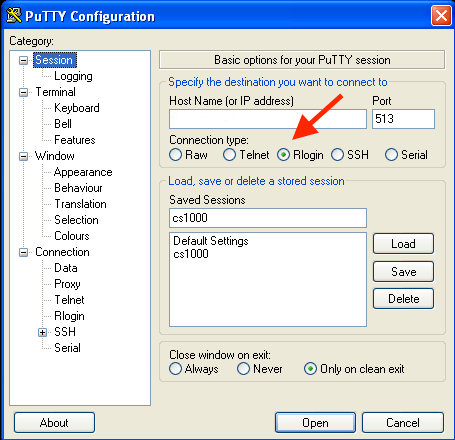
\includegraphics[width=1\textwidth]{figures/rlogin.png}}
\caption{gambar rlogin.}
\label{rlogin}
\end{figure}

\subsection {Tips menggunakan Aplikasi Putty}
Di sini adalah Tips menggunakan Aplikasi Putty dengan mudah
1. Unduh Aplikasi Putty di www.putty.org
2. Jika sudah di unduh, Letakkan Aplikasi Putty.exe ke dalam folder C:\Windows
3. Lalu buat shortcut di desktop dengan klik kanan di desktop lalu add shortcut dan browse aplikasi Putty yang sudah anda unduh
4. Setelah shortcut dibuat, Jalankan Putty.exe dengan klik kanan dan run as administrator.
5. Jika sudah, Lanjut ke pengaturan putty dan atur seperti ini
Mengatur Koneksi Putty :
* Hostname 			: Ip Address
* Port 				: 22
* Connection type 	: SSH
6. Lalu klik Open untuk menjalankan sesi SSH
7. Akan muncul notifikasi bahwa anda untuk pertama kalinya login ke server menggunakan Putty, Pilih Yes untuk melanjutkan.
8. Setelah masuk ke dalam laman awal koneksi SSH Terminal. akan di beri prompt untuk memasukkan username SSH.
9. Lalu masukkan password SSH dan akan nampak ketikan password di terminal tidak terketik. Perlu diingatkan aplikasi terminal tetap menerima ketikan anda walaupun tidak terlihat. Jika masih ragu untuk memasukan password, gunakan Ctrl+C pada bagian kata yang di cap untuk memasukkan password lalu Ctrl+V.
10. Jika sudah memasukkan username dan password SSH, maka anda sudah berhasil login ke server melalui SSH.


